% !TeX root = ../../../main.tex

%************************************************
\chapter{Quantum Chromodynamics}
\label{ch:qcd}
%************************************************
\minitoc
\adjustmtc
\bigskip

\acrfull{qcd} is the theory of strong interactions among colored particles.
It is a fundamental constituent of the \acrfull{sm} of particle physics,
together with the \acrfull{ew} interaction.

The fundamental feature of \qcd is its asymptotic freedom, that makes the
coupling perturbative at high enough energies, but non-perturbative at low
energies, where the relevant scale to compare is the intrinsic
$\Lambda_{\text{QCD}}$, whose order of magnitude is roughly the same of the
mass of the proton ($M_p$).
%
This generates a large amount of composite particles, named \textit{hadrons},
whose constituents are colored particles, i.e.\ quarks, who are determining
main quantum numbers on the hadrons, and gluons, the interaction carrying boson
arising in the corresponding \acrfull{ym} theory, and acting as the binding
glue between quarks.

The discovery of hadrons beyond proton and neutron has driven particle physics
experiments advancements and theoretical progress in the second half of the
twentieth century, resulting in the successful framework of \qcd as a
\acrlong{qft} following the \ym pattern.
But other interesting theories has been investigated during the quest for a
theory of hadrons, and some of them still have relevant consequences, extending
beyond hadrons (e.g.\ string theory, or the old bootstrap).

Despite the success of the framework, the nature of hadrons is still being
intensively investigated, since it would require the solution of
non-perturbative \qcd dynamics.
%
Different tools are available for this investigation, one of them being the
extremely powerful formulation of \qcd on a discretized lattice
\cite{Wilson:1974sk}, but it has not yet been possible to describe the nature
of hadrons from first principles, by a sufficiently accurate lattice
determination.
%
But hadrons are ubiquitous in \hep experiments, both as products of high-energy
collisions, and as scattering particles at hadronic and semihadronic machines,
so a better understanding of the hadronic structure is required to formulate
precise enough theoretical predictions for collision events, confirming in this
way the \sm theory, and investigating possible signals of \acrfull{bsm}
physics.

To circumvent the current limitations about non-perturbative \qft, a different
approach has been pursued, whose origin dates even before the discovery of
\qcd.
In order to analyze collisions of composite particles, it was proposed to
describe them as a packet of collinear point-like constituents, collectively
named \textit{partons}, each one sharing a fraction of the measured momentum of
the scattering particle \cite{Feynman:1969wa}.
%
This partonic picture was successfully applied to predict the high-energy
electron-proton collisions, a process called \acrfull{dis}, resulting in the
discovery of Bjorken scaling \cite{Bjorken:1967fb}, i.e.\ the statement that
\dis structure functions (see \cref{sec:qcd/dis}) do not depend on the
exchanged photon virtuality, setting the energy scale of the process.

Bjorken scaling is then violated by \qcd corrections, but it is still possible
to remain in the framework established by the parton model, because of a
fundamental \qcd property: factorization \cite{Collins:1989gx}.
%
This feature ensures that, up to highly suppressed corrections in the scale
ratio, the hadronic cross-sections factorize in a perturbative hard partonic
cross-sections, that can be computed in perturbation theory with \pqft
calculations, and a universal matrix element, describing the probability that a
certain parton constituent from the original hadron enters the hard event.

It is in this framework that \acrfull{pdf} are defined, as the non-perturbative
matrix element, completing the hadronic cross-section.
\pdf universality ensured by factorization, i.e.\ being independent from the
process considered, makes possible to have a unique set of functions describing
the hadronic structure, bridging the gap from the partonic to the hadronic
cross-sections.
%
In this context, it is possible to avoid the complications of the complexity of
a non-perturbative calculation, resorting on a determination of the \pdf{}s
from experimental data.
In this way, a set of data used to determine the \pdf{}s can constrain the
predictions on other events, including different processes.

\pdf{}s are not the only hadronic object arising from factorization, since also
final products observed in semi-inclusive measurements can be described by
close analogue, called \acrfull{ff}.

More complex object can describe the transverse (non-collinear) dynamics of
partons, like \acrfull{gpd} and \acrfull{tmd}.
Including more degrees of freedom, and requiring the measurement of more
differential observables, the state of this objects is still very raw, compared
to collinear \pdf{}s.
%
The research is actively ongoing in this field, but they will not be further
described in this thesis.

\section{\acrlong{dis}}
\label{sec:qcd/dis}
% % !TeX root = ../../../main.tex

\begin{figure}
	\centering
	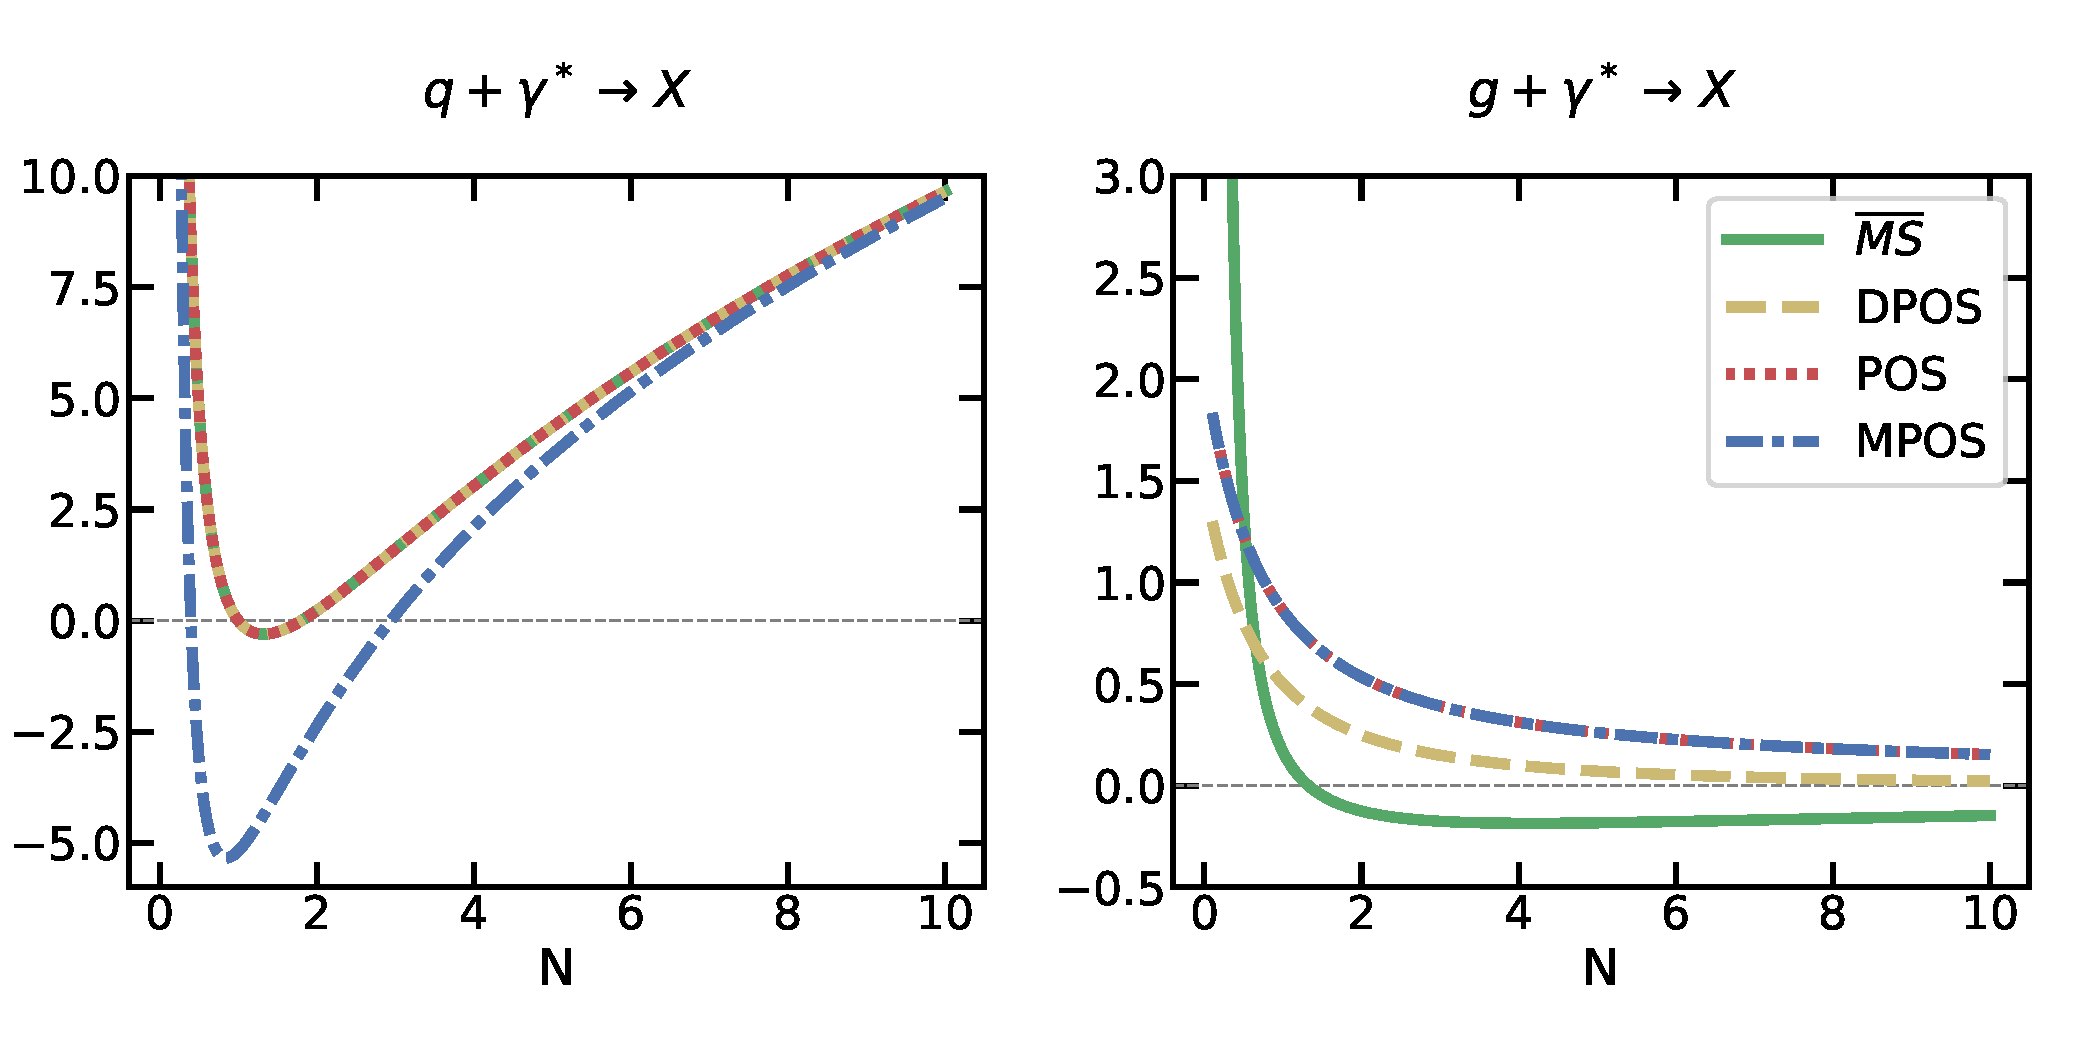
\includegraphics[width=0.6\textwidth]{ch-qcd/dis}
	\caption{
		The \lo Feynman diagram associated to the scattering of a lepton (electron
		in picture) against an hadron component, mediated by an \ew boson.
	}
	\label{fig:qcd/dis}
\end{figure}


The Deep Inelastic Scattering process is the scattering of a lepton over an
hadron component, mediated by an \ew boson \cref{fig:qcd/dis}\footnote{
	This and the other Feynman diagrams in this chapter are taken from the
	\href{https://wiki.physik.uzh.ch/cms/latex:feynman}{related CMS wiki page
		of the Zurich University}.
}.
%
The leptonic part does not couple directly to \qcd , thus the $\alpha_s$
corrections do apply only to the hadronic side (at \lo \ew), and the \ew boson
can be seen as emitted from the incoming lepton and absorbed into the hadron.
%
In this picture the process can be interpreted as the scattering of an
off-shell \ew boson over an hadron, probing the hadron composition.

As discussed in the former section, the history of the \dis process is deeply
connected to the parton model before, and \pdf{}s determination afterwards,
since data from several \dis experiments has been used to provide the main
constraints on the \pdf{}s.
%
Multiple old and more recent \dis experiments are still giving a relevant
contribution to modern datasets used to extract \pdf{}s, including:
\acrfull{slac}, \acrfull{bcdms}, \acrfull{chorus}, \acrfull{nmc}, and the more
recent \nutev.
%
But the \dis data that mostly constrained \pdf{}s have been the results from
\hone and \zeus experiments at \hera.

The entire \cref{ch:dis} will be dedicated to the review of the theory
predictions for this process, and to present a software package, \yadism,
dedicated to the calculation of them, with all relevant variants and options.


\section{Double hadronic \& other processes}
\label{sec:qcd/dy}
% % !TeX root = ../../../main.tex

Until very recently, \dis has been the one process mostly determining \pdf{}s
on its own, even though a non-negligible fraction of \acrfull{ftdy} data was
already included in the main fits.
%
With the advent of the \acrfull{lhc}, this started changing, since the
incredible amount of data generated (and those that will be produced in the
future) are compensating the indirectness of the probe.
%
The \nnpdfr{4.0} release shown for the first time how the \lhc data are not
only giving sizeable contribution to the \pdf{}s determination, but also able
to constraint the \pdf{}s shape on their own \cite{Ball:2021leu}, to a
remarkable degree of accuracy.

\begin{figure}
	\centering
	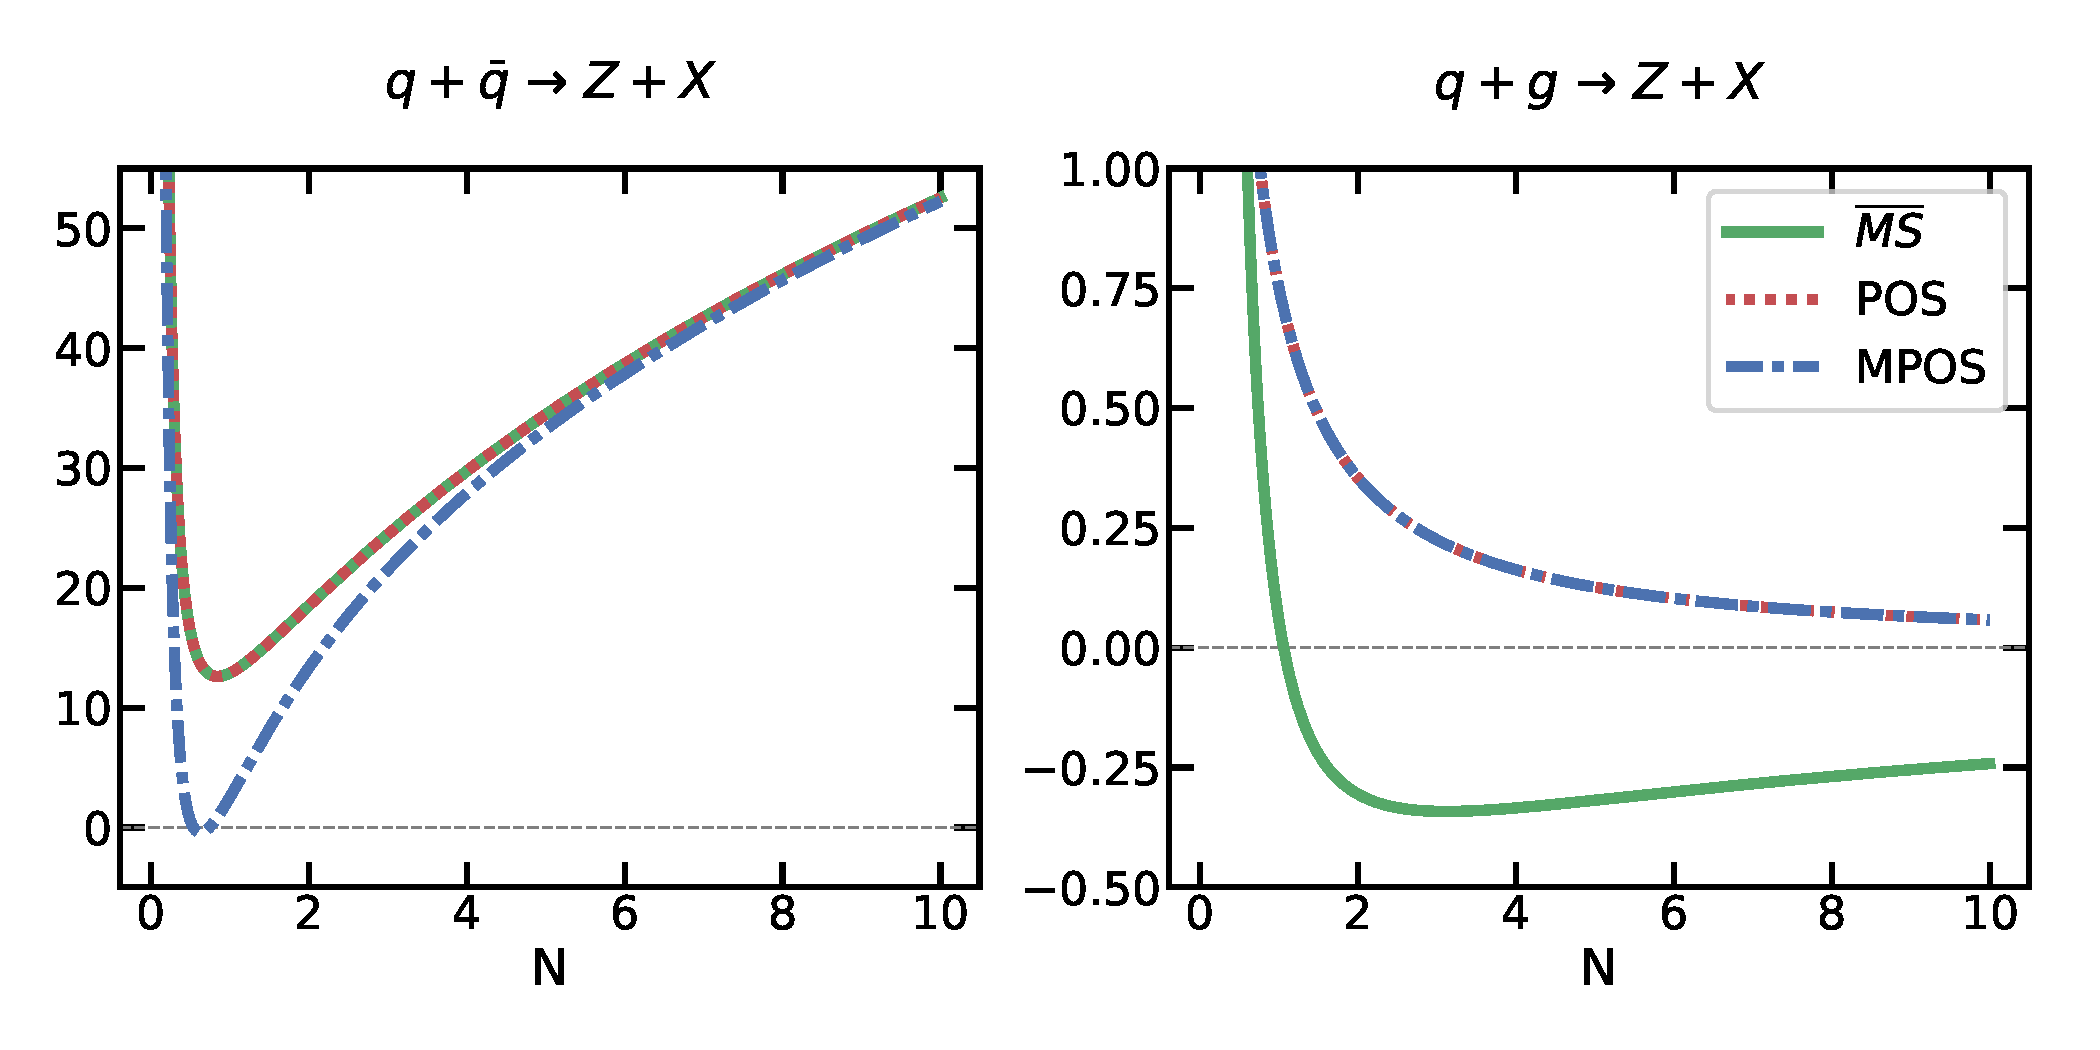
\includegraphics[width=0.6\textwidth]{ch-qcd/dy}
	\caption{
		The \lo Feynman diagram associated to the scattering of two quark
		components of the proton in the $s$-channel, generating a virtual \ew
		boson, eventually decaying leptonically.
	}
	\label{fig:qcd/dy}
\end{figure}

For this reason, double hadronic initiated processes, like $pp$ at \lhc, or
$p\bar{p}$ at \tevatron, are now a relevant part of the global \qcd dataset
used in \pdf{}s extraction.
%
But while for the \dis process analytical calculations are available, most
double hadronic processes require the usage of \acrfull{mc} integrators, since
the resulting integrals are not known analytically, and they quickly extend to
many dimensions.
%
Then, in order to obtain the theory predictions required in \pdf fits, many
different codes are required, since no one implements all possible processes at
the state-of-the-art perturbative order (usually \nnlo by now, but only for
more common processes), and no one is optimal for all of them.

This wide landscape of theoretical predictions, involving increasingly more
demanding software tools, is a challenge for a global \qcd fits, like \pdf
ones, since they will need to interface with a variety of codes constantly
evolving, and find an effective way to decouple the fit itself from the
computational costs involved.
%
This is why interpolation grids have been introduced, to store the results of
\mc computations and offer a unique and fast interface for their consumption.
Grids will be described in more details in \cref{ch:pine}, where a new grid
layout, \pineappl \cite{Carrazza:2020gss}, initially motivated by the extension
of existing formats to allow \ew corrections, has been used to construct a full
pipeline to streamline the process of producing predictions for \pdf and
similar fits.

\begin{figure}
	\centering
	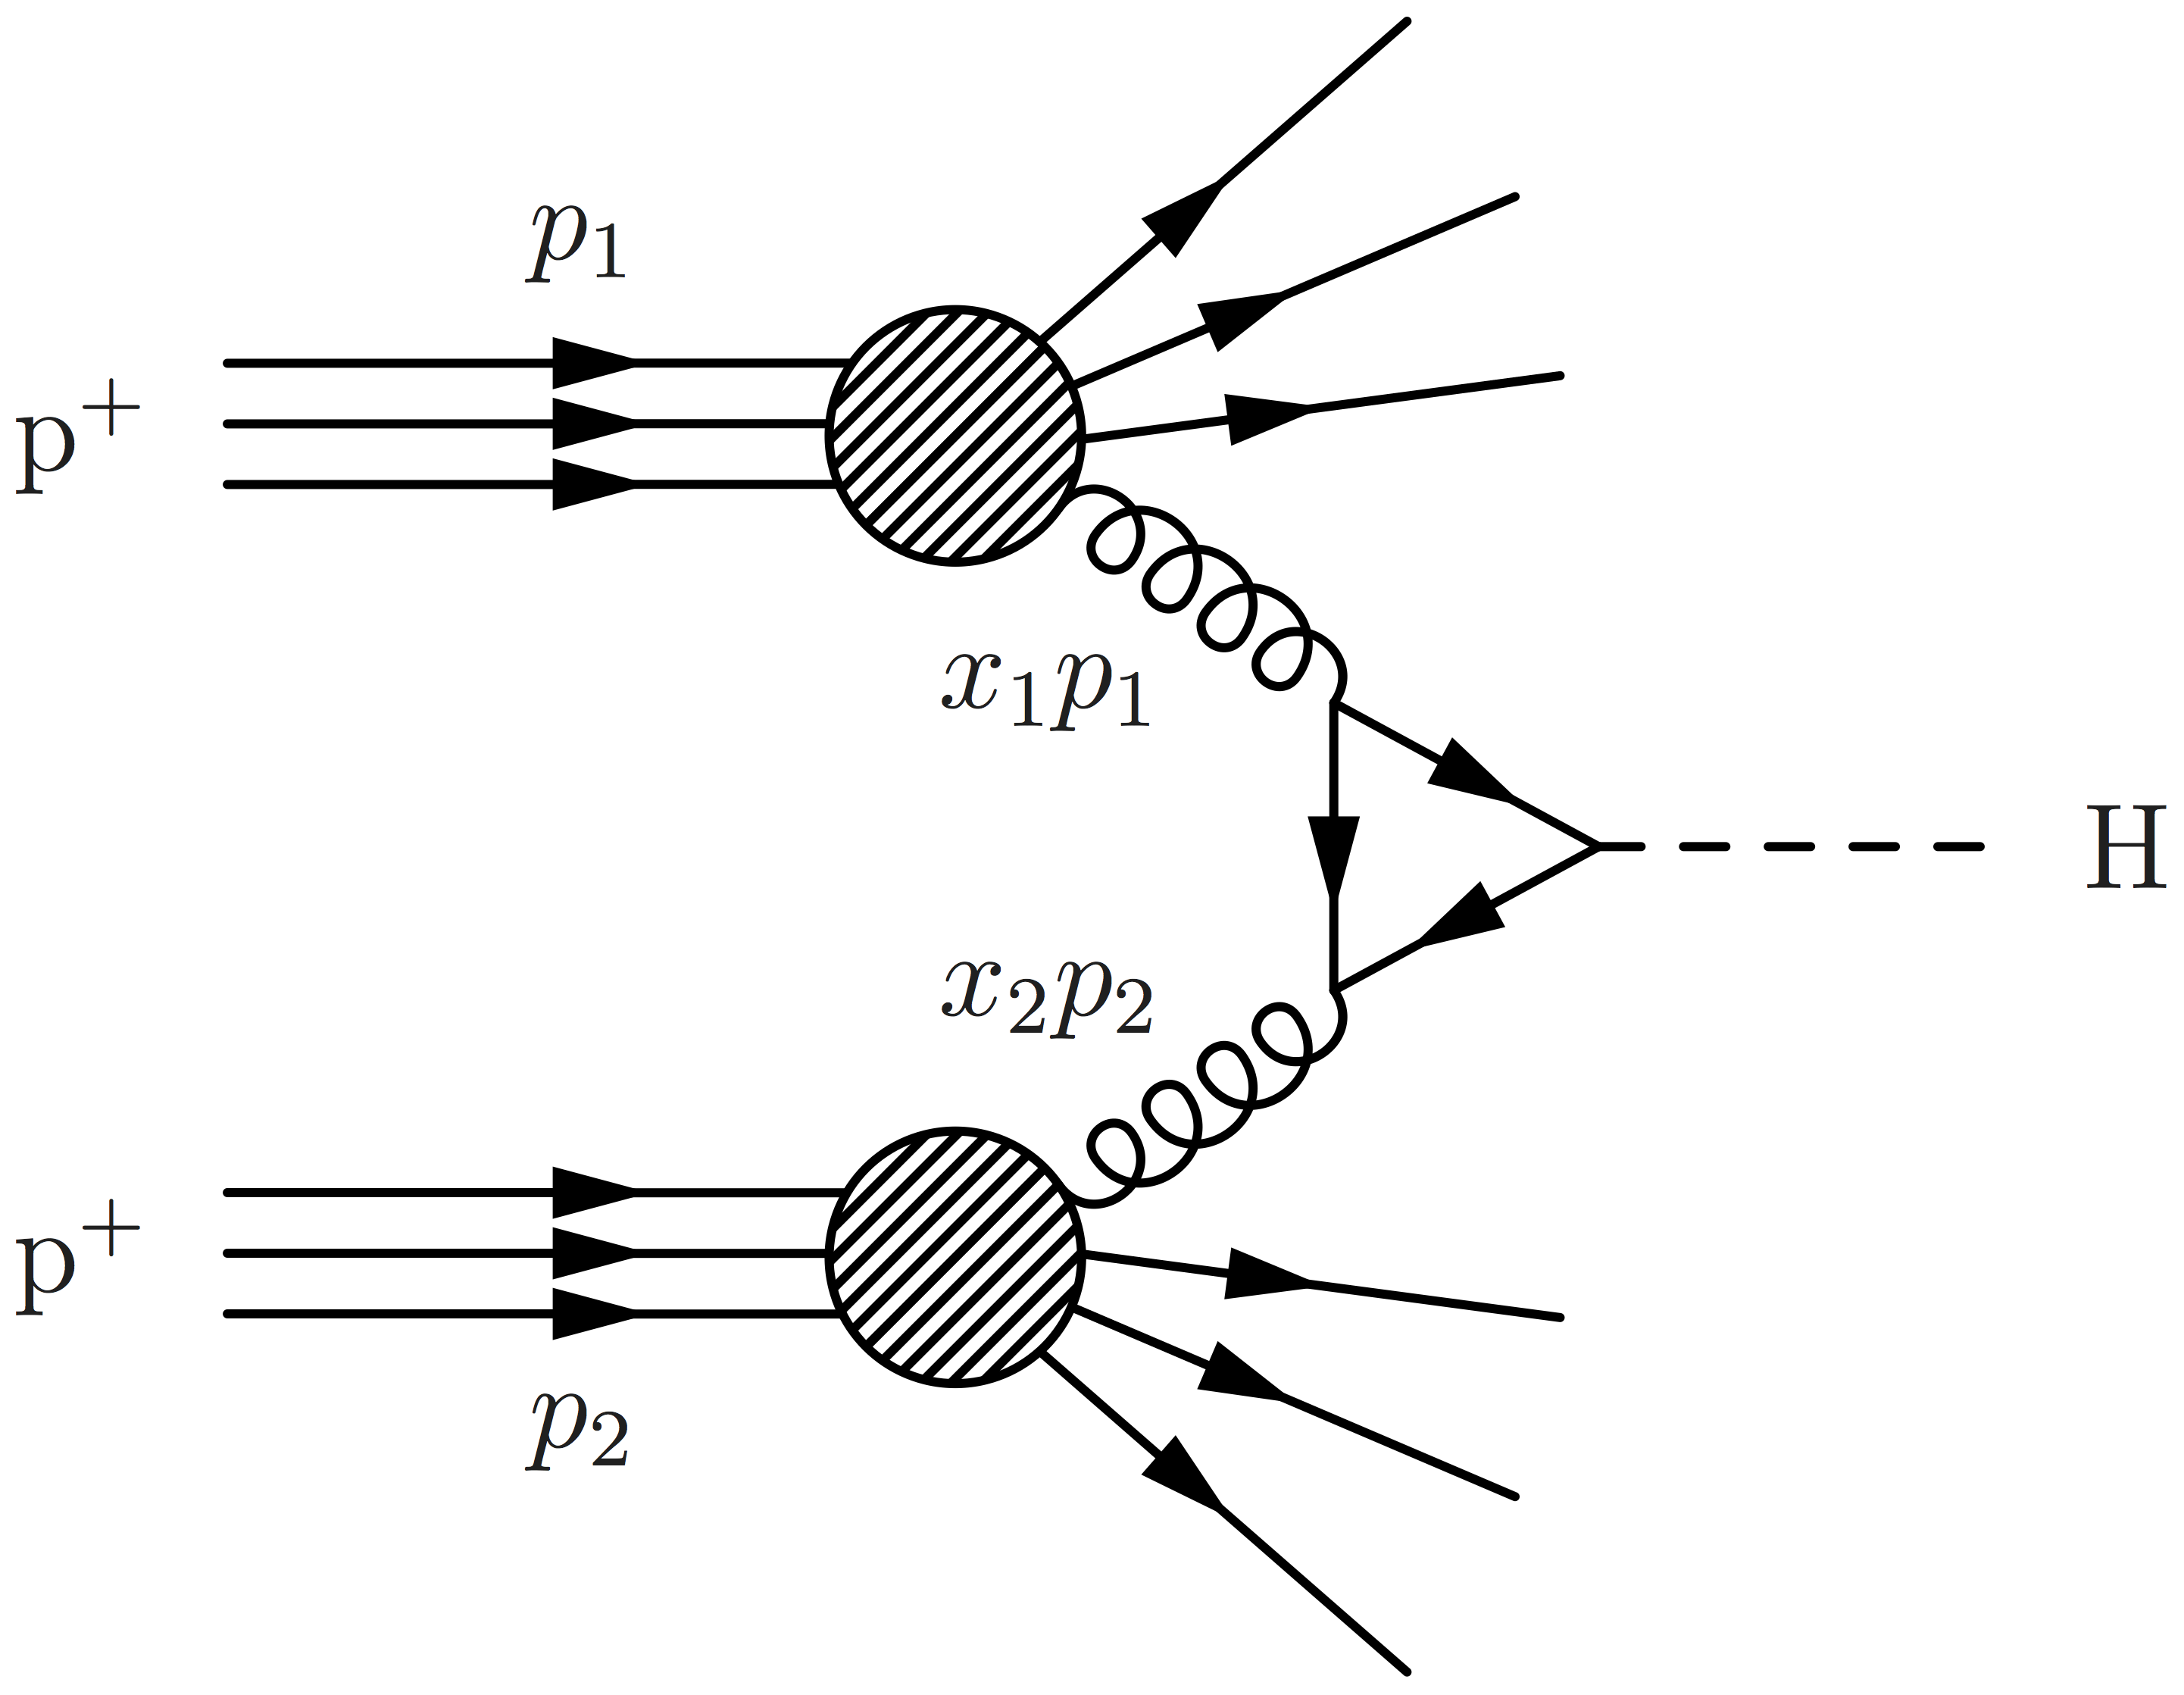
\includegraphics[width=0.6\textwidth]{ch-qcd/ggh}
	\caption{
		The \lo Feynman diagram associated to the scattering of two gluon
		components of the proton, coupling to a virtual quark loop, that
		finally generates an Higgs boson.
		This is the Higgs production via gluon fusion, the main channel for
		Higgs production at \lhc.
	}
	\label{fig:qcd/ggh}
\end{figure}

New processes and observables are being observed at the \lhc, possibly
including new particles and new physics, stressing the need for a more precise
determination of the proton structure.
%
The Higgs production, whose main channel is represented in \cref{fig:qcd/ggh},
that has been first detected by the \lhc collaborations \atlas
\cite{ATLAS:2012yve} and \cms \cite{CMS:2012qbp}, is an extremely well-known
example of new particle discovery, which heavily involved a proton initiated
process, thus depending critically on the \pdf{}s knowledge.


\section{\acrlong{dglap}}
\label{sec:qcd/dglap}
% % !TeX root = ../../../main.tex

\pdfs are a set of functions of two variables (i.e. a function of three
variables, of which one is discrete):
\begin{equation}
  f_i(z, \mu_F^2)
\end{equation}

The three variables are:
\begin{itemize}
  \item the \textit{flavor} $i$ of the chosen parton (usually a \pid in practice)
  \item the \textit{momentum fraction} $z \in (0,1]$ carried by the parton
  \item the \textit{factorization scale} $\mu_F^2 \in \mathbb{R}^+$
\end{itemize}
where the last one is required, since \pdfs are defined through the
factorization theorem, and the factorization scheme used usually involves an
unphysical scale, $\mu_F^2$, in a very similar way to what happens for
renormalization schemes \cite{Ellis:1996mzs}.

The role of the \pdf fits is to determine a border condition at a given value
for the unphysical scale, let it be $\mu_{F,0}^2$, since the dependence on the
scale is fully encoded in perturbative \qcd.
%
Indeed, the various schemes, corresponding to different choices of the
unphysical scale $\mu_F^2$, are related by the analogue of Callan-Symanzik
equations for factorization, obtained asserting that physical observables must
not depend on the choice of the unphysical scale.
%
In such manner, for choices of the scale in the perturbative regime for \qcd,
some terms are factorized either in the \pdf, or in the hard partonic cross
section.
Moving this scale, the terms are swapped, but thus the \pdf values in two
different schemes, corresponding to two different values of the scale, should
compensate for the difference in the partonic cross sections, both obtained by
a perturbative calculation, thus the difference is also determined by
perturbative physics.

This relation between \pdfs defined at different scales takes the shape of a
set of integro-differential equations, called the \acrfull{dglap}
\cite{Altarelli:1977zs,Gribov:1972ri,Dokshitzer:1977sg}:
\begin{equation}
	\muF^2 \dv{\vb f}{\muF^2}{}(x,\muF^2) = \vb P (a_s(\mu^2),\muF^2) \otimes \vb f(\muF^2)
	\label{eq:qcd/dglap}
\end{equation}
The equations establish the anomalous scaling of the \pdfs, and the kernels
${\vb P}$ are called \textit{Altarelli--Parisi splitting functions}.

The equation and its solution is discussed further in \cref{ch:eko}, where
another software package is presented, \eko, automating the solution of the
associated operator equation.
%
Indeed, any linear equation (as \dglap) can be solved by a linear operator,
that is actually producing the solution given any boundary condition, thus
independently of the boundary condition itself:
\begin{equation}
  f_i(z, \mu_F^2) = E_{ij}(\mu_F^2 \gets \mu_{F,0}^2) \otimes f_j(\mu_{F,0}^2)
\end{equation}
We call such an operator, for \dglap, \acrfull{eko}.

This is another central ingredient in \pdf fits, since the data set span
different scales, over multiple order of magnitudes, so the \pdf determined by
the fit has to be evolved first to the suitable scale, to be folded with the
partonic calculation at that scale, resulting in the hadronic predictions for
the measured observable.


